\documentclass[11pt,a4paper,headinclude,footinclude,DIV16,normalheadings]{scrreprt}
\usepackage[automark]{scrpage2}
\usepackage[ansinew]{inputenc}
\usepackage{amsmath}
\usepackage{amsfonts}
\usepackage{theorem}
\usepackage{color}
\usepackage{listings}
\lstset{language=C++, basicstyle=\ttfamily, 
  keywordstyle=\color{black}\bfseries, tabsize=4, stringstyle=\ttfamily,
  commentstyle=\it, extendedchars=true, escapeinside={/*@}{@*/}}
\usepackage{hyperref}
\usepackage{psfrag}
\usepackage{makeidx}
\usepackage{graphicx}
\usepackage[htt]{hyphenat}
\usepackage{color}

\DeclareGraphicsExtensions{.eps, .jpg}

\newcommand{\Dune}{{\sf\bfseries DUNE}}
\newcommand{\Dumux}{DuMu$^\text{x}$ }

%The theorems
\theorembodyfont{\upshape}
\theoremheaderfont{\sffamily\bfseries}
\newtheorem{exc}{Exercise}[chapter]
\newtheorem{rem}[exc]{Remark}
\newtheorem{lst}{Listing}
\newtheorem{warn}[exc]{Warning}

\pagestyle{scrheadings}

\title{\Dumux Handbook}

\author{}

\date{\today}

\publishers{%
\vspace{10mm}
{\normalsize Lehrstuhl f\"ur Hydromechanik und Hydrosystemmodellierung, \\
Universit\"at Stuttgart, Paffenwaldring 61, D-70569 Stuttgart, Germany}\\
%
\bigskip
{\normalsize \texttt{\url{http://www.dumux.uni-stuttgart.de}}}\\
}

\makeindex

\begin{document}

\maketitle

\begin{abstract}

\end{abstract}

\tableofcontents

\chapter{Introduction}

\eWoms~\cite{EWOMS-HP} a generic simulation framework using continuum
mechanical approaches with a focus on multi-phase fluid flow and
transport processes in porous media. \eWoms is also an integral part
of the open porous media initiative~\cite{OPM-HP} for which it
implements the fully-implicit discretization schemes. \eWoms is based
on the source code of the \Dumux~\cite{DUMUX-HP} simulation framework
and aims to be a proper superset of \Dumux when it comes to features,
while at the same time it delivers better performance and a
higher-quality code base. To ease porting features from \Dumux to
\eWoms, the \eWoms source code uses very similar naming and style
conventions as the one of \Dumux.

Besides being a generic simulation framework, \eWoms also aims to to
deliver top-notch computational performance, high flexibility, a sound
software architecture and the ability to run on anything from single
processor systems to highly parallel supercomputers with specialized
hardware architectures. The means to achieve these somewhat
contradictory goals are the thorough use of object oriented design in
conjunction with template programming. These requirements motivated
the decision to implement \eWoms using the \Cplusplus programming
language.

One of the more complex issues when dealing with parallel continuum
models for partial differential equations, is the management of the
grids used for the spatial discretization. To date, no generic and
efficient approach exists for all possible cases, which lead to \eWoms
being build on top of \Dune, the \textbf{D}istributed and
\textbf{U}nified \textbf{N}umerics
\textbf{E}nvironment~\cite{DUNE-HP}. Instead of trying to implement a
grid for everything, \Dune defines a generic \Cplusplus interface to
grids, and provides adapters to several existing grid management
libraries such as UG~\cite{UG-HP}, ALBERTA~\cite{ALBERTA-HP} or
ALUGrid~\cite{ALUGRID-HP}. DUNE also extensively uses template
programming in order to achieve minimal overhead when accessing the
underlying grid libraries\footnote{In fact, the performance penalty
  resulting from the use of \Dune's grid interface is usually
  negligible~\cite{BURRI2006}.}.
\begin{figure}[hbt]
  \centering
  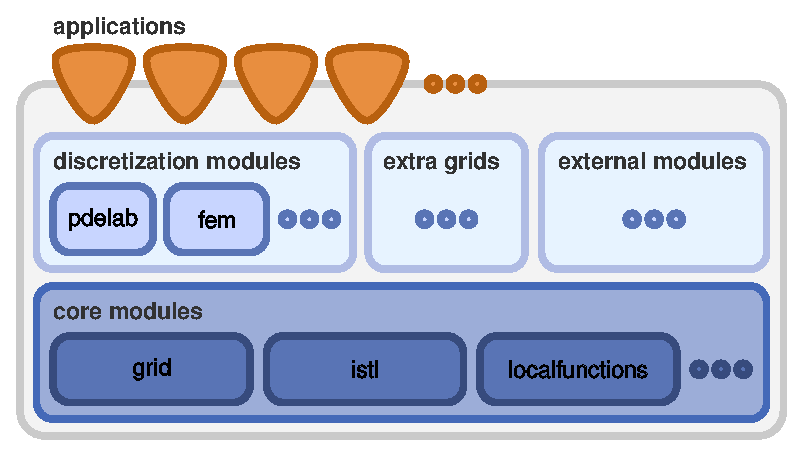
\includegraphics[width=.5\linewidth, keepaspectratio]{EPS/dunedesign}
  \caption{
    \label{fig:dune-design}
    A high-level overview of \Dune's design is available on the project's
    web site~\cite{DUNE-HP}.
  }
\end{figure}

DUNE's grid interface is independent of the spatial dimension of the
underlying grid. For this purpose, it uses the concept of
co-dimensional entities. Roughly speaking, an entity of co-dimension
$0$ constitutes a cell, co-dimension $1$ entities are faces between
cells, co-dimension $1$ are edges, and so on until co-dimension $n$
which are the cell's vertices.  The \Dune grid interface generally
assumes that all entities are convex polytopes, which means that it
must be possible to express each entity as the convex hull of a set of
vertices. For the sake of efficiency, all entities are further expressed in terms
of so-called reference elements which are transformed to the actual
spatial incarnation within the grid by a so-called geometry
function. Here, a reference element for an
entity can be thought of as a prototype for the actual grid
entity. For example, if we used a grid which applied hexahedrons as cells,
the reference element for each cell would be the unit cube $[0, 1]^3$
and the geometry function would scale and translate the cube so that
it matches the grid's cell. For a more thorough description of \Dune's
grid definition, see~\cite{BASTIAN2008}.

In addition to the grid interface, \Dune also provides quite a few
additional modules; In the context of this handbook the
\texttt{dune-localfunctions} and \texttt{dune-istl} modules are
probably the most relevant. \texttt{dune-localfunctions} provides a
set of generic finite element shape functions, while
\texttt{dune-istl} is the \textbf{I}terative \textbf{S}olver
\textbf{T}emplate \textbf{L}ibrary and provides generic, highly
optimized linear algebra routines for solving linear systems of
equations.

\eWoms comes in form of a module \Dune module '\texttt{ewoms}'.  It
depends on the \Dune core modules \texttt{dune-common},
\texttt{dune-grid}, \texttt{dune-istl}, and on
\texttt{dune-localfunctions}.  The main intention of \eWoms is to
provide a framework for an easy and efficient implementation of new
physical models for porous media flow problems, ranging from problem
formulation and the selection of spatial and temporal discretization
schemes as well as nonlinear and linear solvers, to general concepts
for model coupling.  Moreover, \eWoms includes ready-to-use numerical
models and a few example applications.

%%% Local Variables:
%%% mode: latex
%%% TeX-master: "ewoms-handbook"
%%% End:

\chapter{Set-up and basic workflows}

This chapter is aimed at setting up a development environment for
\eWoms and to equip you with a rough understanding of the basic
workflows used for developing the software. We will first have a
brief look at the installation procedure; After that, we will run a
sample simulation and briefly discuss how to visualize its results.

Be aware, that this is only a very streamlined version of the \eWoms
development workflow, so make yourself confident with the tools
introduced in this section before you delve into the \Cplusplus code
in the next chapter.

\section{Quick Installation of \eWoms} \label{quick-install}

This only provides one quick way of installing \eWoms.  As a
pre-requisite it is assumed that you are using \eWoms with a recent
Linux distribution that has the appropriate development packages
installed, but without the distribution packages of the \Dune core
modules installed.  If you need more information, or if you have \Dune
already installed, please have a look at the detailed installation
instructions in Section \ref{install}.

\subsection{Retrieving the code}


You can download all \Dune modules by either downloading and unpacking
the tarballs for the \Dune-2.2 release as well as downloading and
unpacking the tarball for the \eWoms 2.2 release, or by retrieving the
code directly from their respective source-code repositories. If you
decide to use the first method, make sure to unpack all tarballs into
the same directory, for the second method you can enter the following
code snipplet into a terminal:
\begin{lstlisting}[style=Bash]
for DUNE_MODULE in common geometry grid istl localfunctions; do \
     git svn clone https://svn.dune-project.org/svn/dune-$DUNE_MODULE/branches/release-2.2 $DUNE_MODULE \
done
git clone --branch "release-2.2" git://github.com/OPM/ewoms.git
\end{lstlisting}

\subsection{Building \Dune and \eWoms}
\label{buildIt}

\eWoms is (almost) a standard \Dune module and is recommended to be
build using the \Dune build system~\cite{DUNE-BS}. \eWoms ships with a
few option files for \Dune's build script, \texttt{dunecontrol}. For
the first time compilation we recommend to use the options optimized
for the debugging experience, \texttt{debug.opts}:

\begin{lstlisting}[style=Bash]
# make sure you are in the DUNE's root directory 
./dune-common/bin/dunecontrol --opts=ewoms/debug.opts all
\end{lstlisting}

If you finished with developing and testing your own code on
small-scale problems, re-compile everything with compiler
optimizations enabled before a production run:

\begin{lstlisting}[style=Bash]
# make sure you are in the DUNE's root directory
./dune-common/bin/dunecontrol --opts=ewoms/optim.opts all
\end{lstlisting}

Sometimes it is necessary to have additional options which are
specific to the concrete operating system you use or you might also
have special needs.  For this reason, the option files mentioned above
are to be rather understood as a starting point for specifying the own
options than as something which is fixed; feel free to copy and modify
them.  For example, if you need external libraries, you might need to
add or modify quite many options.  To avoid confusion, it can also be
helpful to use a different name for your customized option files.

%%% Local Variables: 
%%% mode: latex
%%% TeX-master: "ewoms-handbook"
%%% End: 

\section[Quick start guide]{Quick start guide: The first run of a test application}\label{quick-start-guide}

The previous chapter showed, how to install and compile \Dumux. This chapter shall give a very brief introduction, how to run a first test application and how to visualize the first output files. Only the rough steps will be described here. More detailed explanations can be found in the tutorials in the following chapter.

\begin{enumerate}
 \item Go to the directory \texttt{/test}. There, various test application folders can be found. Let us consider as example \texttt{boxmodels/test{\_}2p}:
 \item Enter the folder \texttt{boxmodels/2p}. If everything was compiled correctly, there should be an executable \texttt{test{\_}2p}. Otherwise, type \texttt{make test{\_}2p} in order to compile the application. To run the simulation, type\\ 
\texttt{./test{\_}2p 1e4 1e2}\\
into the console. The parameters that are used here are the end time of the simulation and the initial timestep size. The parameters that are required when calling the application are specified in the application file (here: test{\_}2p.cc).
 \item The simulation starts and produces some .vtu output files and also a .pvd file. The .pvd file can be used to examine time series and summarizes the .vtu-files. It is possible to stop a running application by pressing $<ctrl><c>$.
 \item You can display the results using the visualization tool ParaView (or alternatively VisIt). Just type \texttt{paraview} in the console and open the .pvd file. On the left hand side, you can choose the desired parameter to be displayed.
\end{enumerate}
% 
%
%



\section{Specifying Parameters}
\label{sec:inputFiles}

As already mentioned in the previous section, \eWoms allows to specify
a number of parameters at run time. A description of these parameters
can usually obtained by passing the \texttt{--help} parameter to the
executable. The values used for these parameters are printed to the
terminal during the start-up of the simulation, e.g. the if the \texttt{lens\_immiscible}
simulation is run with the parameters \texttt{--end-time=30e3 --foo-param=123}, there will an output similar to
\begin{lstlisting}[style=Bash]
###########
# Parameters specified at run-time
###########
EndTime="30e3"
###########
# Parameters with use compile-time fallback values
###########
AmgCoarsenTarget="5000"
...
VtkWriteSaturations="1"
VtkWriteTemperature="1"
VtkWriteViscosities="0"
###########
# Parameters unknown to the simulation
###########
FooParam="123"
\end{lstlisting}

This can be directly copy-and-pasted into a file
(e.g. \texttt{myparams.ini}) and loaded by passing the
\texttt{--parameter-file=myparams.ini} parameter to the simulation the
next time it is run.

When you do simulations, always look for the paramters which are
unknown to the simulation, as this is \emph{very} useful for spotting
typos.

%%% Local Variables: 
%%% mode: latex
%%% TeX-master: "ewoms-handbook"
%%% End: 


%%% Local Variables:
%%% mode: latex
%%% TeX-master: "ewoms-handbook"
%%% End:

\chapter[Tutorial]{Tutorial}\label{chp:tutorial}

In \Dumux two sorts of models are implemented: Fully-coupled models and decoupled models. In the fully-coupled models a flow system is described by a system of strongly coupled equations which can be mass balance equations, balance equations of components, energy balance equations, etc. In contrast a decoupled model consists of a pressure equation which is iteratively coupled to a saturation equation, concentration equations, energy balance equations, etc.

Examples for different kinds of both coupled and decoupled models are isothermal two-phase models, isothermal two-phase two-component models, non-isothermal two-phase models, non-isothermal two-phase two-component models, etc.

In section \ref{box} a short introduction about the box method is given. The box method is used for the spatial discretization of the system of equations. The other two sections of the tutorial demonstrate how to solve problems first using a coupled model (section \ref{tutorial-coupled}) and second using a decoupled model (section \ref{tutorial-decoupled}). Being the easiest case, an isothermal two-phase system (two fluid phases, one solid phase) will be considered.
\clearpage
\section[Fully-coupled model]{Solving a problem using a Fully-Coupled Model}\label{tutorial-coupled}

The process of solving a problem using \Dumux can be roughly divided into four parts:
\begin{enumerate}
 \item The geometry of the problem and correspondingly a grid have to be defined.
 \item Material properties and constitutive relationships have to be defined.
 \item Boundary conditions as well as initial conditions have to be defined.
 \item A suitable model has to be chosen.
\end{enumerate}

The problem that is solved in this tutorial is illustrated in figure \ref{tutorial-coupled:problemfigure}. A rectangular domain with no flow boundaries on the top and on the bottom, which is initially saturated with oil, is considered. Water infiltrates from the left side into the domain. Gravity effects as well as capillarity effects are neglected.

\begin{figure}[h]
\psfrag{x}{x}
\psfrag{y}{y}
\psfrag{no flow}{no flow}
\psfrag{water}{\textbf{water}}
\psfrag{oil}{\textcolor{white}{\textbf{oil}}}
\psfrag{p_w = 2 x 10^5 [Pa]}{$p_w = 2 \times 10^5$ [Pa]}
\psfrag{p_w_initial = 2 x 10^5 [Pa]}{\textcolor{white}{\textbf{$\mathbf{p_{w_{initial}} = 2 \times 10^5}$ [Pa]}}}
\psfrag{S_n = 0}{$S_n = 0$}
\psfrag{S_n_initial = 0}{\textcolor{white}{$\mathbf{S_{n_{initial}} = 1}$}}
\psfrag{q_w = 0 [kg/m^2s]}{$q_w = 0$ $\left[\frac{\textnormal{kg}}{\textnormal{m}^2 \textnormal{s}}\right]$}
\psfrag{q_n = -3 x 10^-4 [kg/m^2s]}{$q_n = -3 \times 10^-4$ $\left[\frac{\textnormal{kg}}{\textnormal{m}^2 \textnormal{s}}\right]$}
\centering
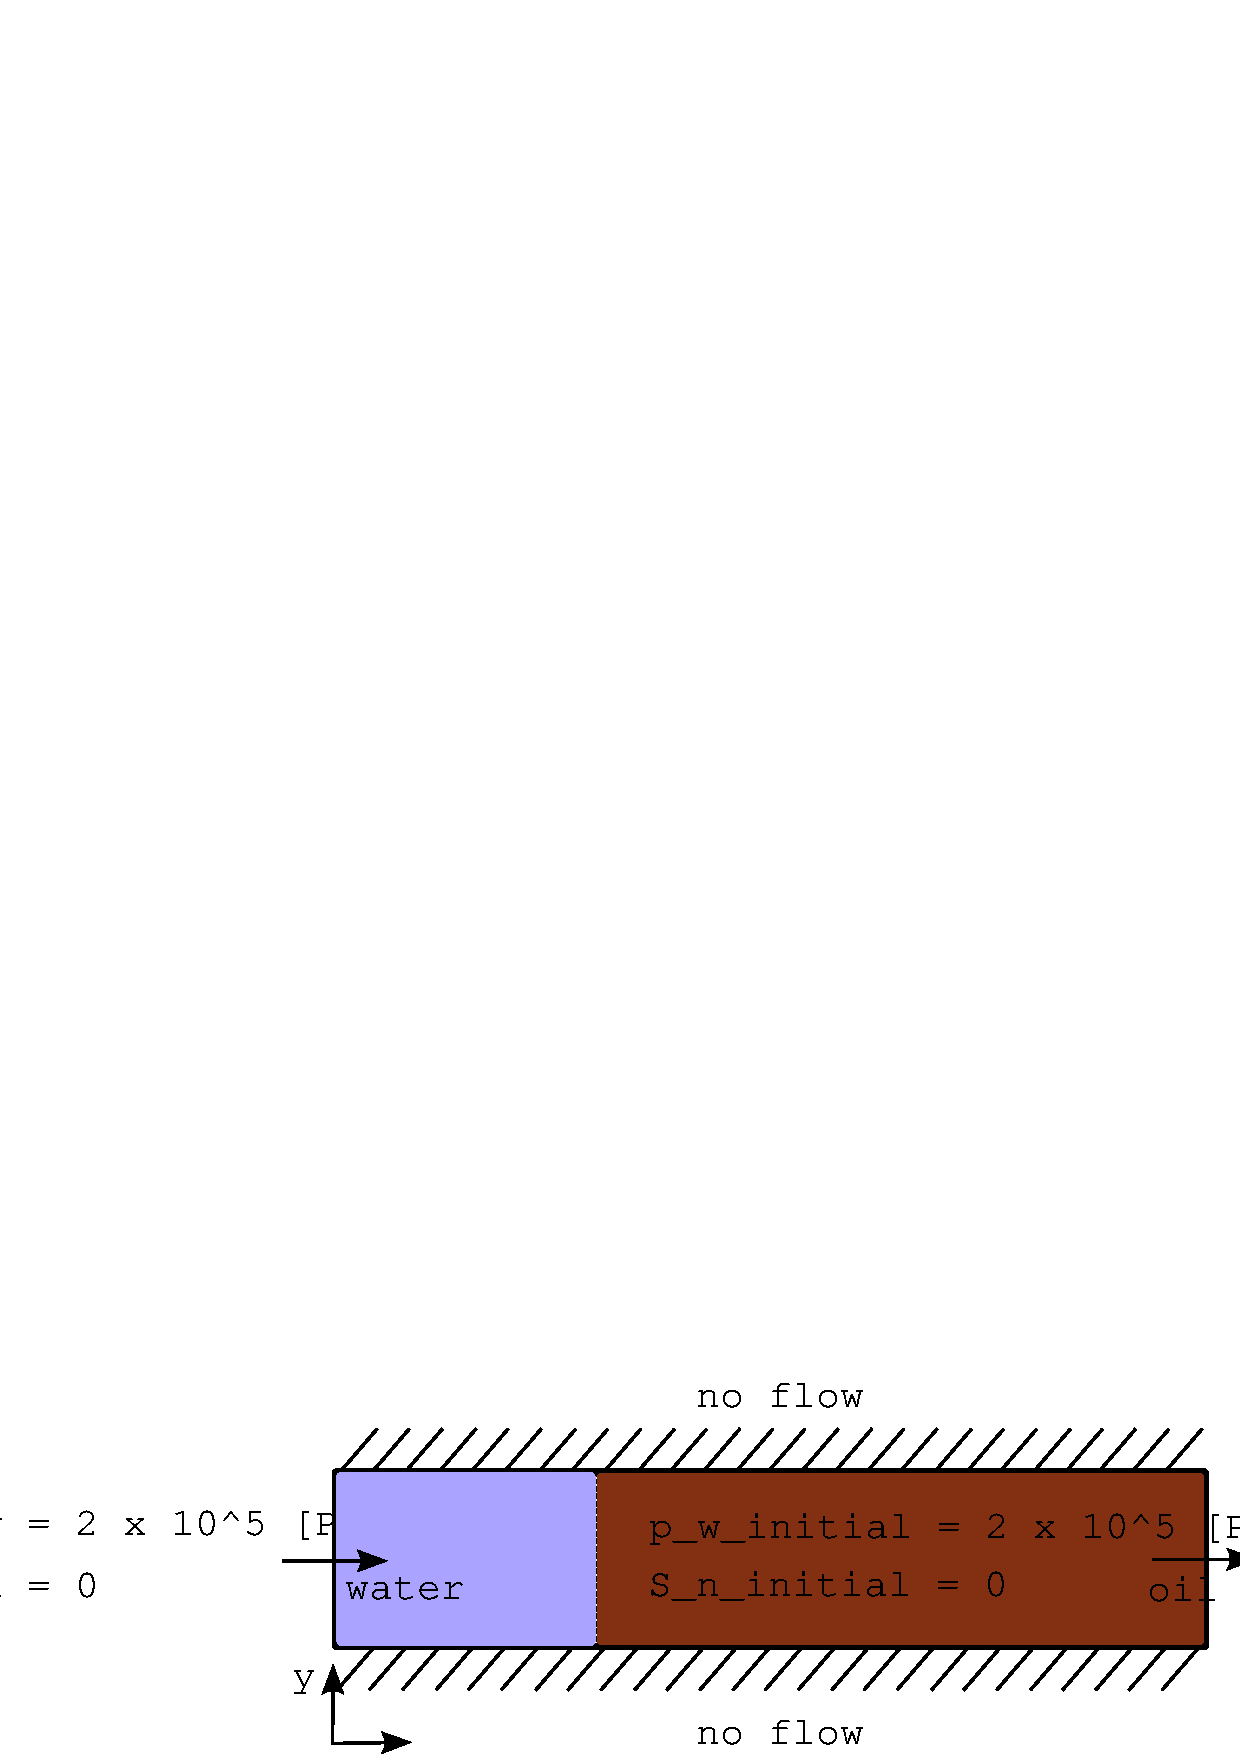
\includegraphics[width=0.9\linewidth,keepaspectratio]{EPS/tutorial-problemconfiguration}
\caption{Geometry of the tutorial problem with initial and boundary conditions.}\label{tutorial-coupled:problemfigure}
\end{figure}

Listing \ref{tutorial-coupled:mainfile} shows the main file \texttt{tutorial\_coupled.cc} for the coupled twophase model. This file needs to be executed to solve the problem described above. The main file can be found in the directory \texttt{/dune-mux/test/tutorial}.

\begin{lst}[File dune-mux/test/tutorial/tutorial\_coupled.cc]\label{tutorial-coupled:mainfile} \mbox{}
\lstinputlisting[basicstyle=\ttfamily\scriptsize,numbers=left,
numberstyle=\tiny, numbersep=5pt]{../../test/tutorial/tutorial_coupled.cc}
\end{lst}

From line \ref{tutorial-coupled:include-begin} to line \ref{tutorial-coupled:include-end} the Dune and the \Dumux files which contain the functions and classes that are needed in the main function are included into the main file.

The geometry of the problem and the grid on which the problem is to be solved are defined in the lines \ref{tutorial-coupled:grid-begin} to \ref{tutorial-coupled:grid-end}. The three variables of Type \texttt{Dune::FieldVector} define the lower left corner of the domain (\texttt{L}), the upper right corner of the domain (\texttt{H}) and the number of cells in $x$ and $y$ direction (\texttt{N}). The dimension \texttt{dim} is previously defined in line \ref{tutorial-coupled:dim}. The grid of type \texttt{Dune::SGrid} is then generated in line \ref{tutorial-coupled:grid-end}. For more information about the dune grid interface, the different grid types that are supported and the generation of different grids it is referred to the \textit{Dune Grid Interface HOWTO (http://www.dune-project.org/doc/)}.

The second step needed to solve the problem is the definition of material properties and constitutive relationships. The fluid properties of the two fluid phases considered here are defined in the lines \ref{tutorial-coupled:water} and \ref{tutorial-coupled:oil}. \Dumux provides several fluid classes which can be found in the file \texttt{phaseproperties2p.hh} in the directory \texttt{/dune-mux/dumux}-\texttt{/material/phaseproperties}. \\
The properties of the solid matrix are defined in a special soil class. The \texttt{soil} object is generated in line \ref{tutorial-coupled:soil}. As can be seen, the class type is \texttt{Dune::TutorialSoil}, which is defined in the file \texttt{tutorial\_soilproperties.hh} in the folder \texttt{/test/tutorial}. A description of this file and the definition of a soil class including the soil parameters can be found in section \ref{tutorial-coupled:description-soil-class}. Finally, in line \ref{tutorial-coupled:twophaserelations} the information included in the fluid and soil objects is used to generate an object of type \texttt{Dune::TwoPhaseRelations}, which includes the constitutive relationships (capillary pressure-saturation relation, relative permeability-saturation relation, etc.). The file \texttt{twophaserelations.hh} can be found in the directory \texttt{/dune-mux/dumux/material}.

The definition of boundary and initial conditions as well as source or sink terms is done by definition of a so-called \textit{problem} class. In case of this tutorial the problem class is defined in the file \texttt{tutorialproblem\_coupled.hh} in the \texttt{/test/tutorial} folder. In the main file the problem object of type \texttt{Dune::TutorialProblemCoupled} is then generated in line \ref{tutorial-coupled:problem}. A further explanation of the definition of boundary and initial conditions, source and sink terms and the structure of the problem class can be found in section \ref{tutorial-coupled:description-bc-ic}. Besides the definition of the boundary and initial conditions the problem class is also a kind of interface containing all the objects generated before (geometry, fluids, soil, constitutive relationships, etc.). Thus, as can be seen in line \ref{tutorial-coupled:problem} all this objects are given as arguments when calling the constructor of the problem class.     

Finally, a numerical model has to be chosen that defines how the coupled system of equations is discretized. In case of this tutorial a coupled isothermal two phase model is the choice. A coupled model may consist of two or more mass balance equations and if required an energy balance equation. For the given example problem of a pure isothermal two phase flow. A coupled system of two equations is solved. 
%The two equations are given below:
%\begin{equation}
%\end{equation}
%GLEICHUNGEN\\
%ERKLAERUNG ZU BOX\\

The discretisation of these equations is included in the object which is generated in line \ref{tutorial-coupled:boxmethod} of the main file. It is called \texttt{boxmethod} and it is of type \texttt{Dune::BoxPwSn}. The definition of this class can be found in \texttt{/dune-mux/dumux/twophase/fv} in the file \texttt{boxpwsnjacobian.hh}. The \texttt{Box} in the class name indicates that the \textit{boxmethod} is used for the discretisation. 

Finally, an object called \texttt{timeloop} of type \texttt{Dune::TimeLoop} is generated in line \ref{tutorial-coupled:timeloop} of the tutorial main file. The class \texttt{Dune::TimeLoop} is defined in the file \texttt{timeloop.hh} in the folder \texttt{/dune-mux/dumux/timedisc}. The object \texttt{timeloop} includes the type of timestep that is used (implicit, explicit, etc.) and contains the function \texttt{execute} which is called in line \ref{tutorial-coupled:execute} of the main file. This function finally starts the computation and runs the (time)loop over all timesteps.

\subsection{The definition of the fluid properties}\label{tutorial-coupled:description-fluid-class}

In \Dumux different fluids are already implemented. The definitions can be found in the file \texttt{phaseproperties2p.hh} in the directory \texttt{/dune-mux/dumux/material/phaseproperties}. In this file, for each fluid a class named like the fluid is defined. These classes are derived from the fluid base class \texttt{Fluid} which is defined in the file \texttt{property\_baseclasses.hh} in the directory \texttt{/dune-mux/dumux/material} and include several functions returning different fluid properties. New fluids which are not yet available in the file \texttt{phaseproperties2p.hh} can be defined here accordingly.

It is important to mention, that existing fluid classes should not be changed. New fluid classes should only be added to the file \texttt{phaseproperties2p.hh} if they are also to be added to the repository! If you are not sure if your fluid class can be useful for the other \Dumux users just create a new file in your problem directory similar to the file \texttt{phaseproperties2p.hh} and define your fluid classes there.

\subsection{The definition of the soil parameters}\label{tutorial-decoupled:description-soil-class}

Soil properties which can be defined in \Dumux are the \textit{intrinsic permeability}, the \textit{porosity} and the \textit{heat capacity} as well as the \textit{heat conductivity} of the solid matrix. Further the \textit{residual saturations} of the fluids, and the \textit{capillary pressures-saturation function} as well as the \textit{relative permeability-saturation functions} are depending on the soil.

The base class \texttt{Dune::Matrix2p} for the definition of the soil parameters can be found in the file \texttt{property\_baseclasses.hh} in the directory \texttt{/dune-mux/dumux/material}. Derived from this base class, there exist two standard soil type classes named \texttt{HomogeneousSoil} and \texttt{HeterogeneousSoil}. Both can be found in the file \texttt{matrixproperties.hh} in the \texttt{/material} folder. If one wants to use a soil that differs from this standard soil types, new soil classes can be derived either from the base class (\texttt{Dune::Matrix2p}) or from the two standard soil classes (\texttt{Dune::HomogeneousSoil} and \texttt{Dune::HeterogeneousSoil}).

For this tutorial problem a new soil class named \texttt{TutorialSoil} is derived from \texttt{Dune::HomogeneousSoil} (listing \ref{tutorial-decoupled:soilpropertiesfile}, line \ref{tutorial-decoupled:tutorialsoil}), which can be found in the file \texttt{tutorial\_soilproperties.hh} in the directory \texttt{/test/tutorial}.

Listing \ref{tutorial-decoupled:soilpropertiesfile} shows the file \texttt{tutorial\_soilproperties.hh}.

\begin{lst}[File dune-mux/test/tutorial/tutorial\_soilproperties.hh]\label{tutorial-decoupled:soilpropertiesfile} \mbox{}
\lstinputlisting[basicstyle=\ttfamily\scriptsize,numbers=left,
numberstyle=\tiny, numbersep=5pt]{../../test/tutorial/tutorial_soilproperties.hh}
\end{lst}

In line \ref{tutorial-decoupled:permeability} the function returning the intrinsic permeability can be found. As can be seen, the function has to be called with three different arguments. The first one (\texttt{x}) is a vector including the global coordinates of the current entity (can be an element, vertex, etc.), the second one (\texttt{e}) is the entity itself and the third one is a vector including the local coordinates of the current entity. The intrinsic permeability is a tensor and thus returned in form of a $n \times n$-matrix where $n$ is the dimension of the problem.

The function \texttt{porosity()} defined in line \ref{tutorial-decoupled:porosity} is called with the same arguments as the permeability function described before and returns the porosity dependent on the position in the domain.

The residual saturation functions \texttt{Sr\_w()} (line \ref{tutorial-decoupled:srw}) and \texttt{Sr\_n()} (line \ref{tutorial-decoupled:srn}) additionally have the temperature as function argument, which is set to a default value if an isothermal model is used.

Finally, the functions defining the type of the capillary pressure function and the relative permeability functions have to be considered. In line \ref{tutorial-decoupled:flags} the function \texttt{relPermFlag()} is defined. This function returns a flag indicating the type of function which is used depending on the position. This could be a linear function, a \textit{Brooks-Corey} function, a \textit{van Genuchten} function, etc. The flags that can be chosen as return parameter are defined in the base soil class \texttt{Matrix2p} in the file \texttt{property\_baseclasses.hh}. The parameters used in the chosen function type can be defined in the function \texttt{paramRelPerm} (line \ref{tutorial-decoupled:parameters}). As can be seen in listing \ref{tutorial-decoupled:soilpropertiesfile}, e.g. linear capillary pressure and relative permeability functions require a vector of two arguments, one defining the minimum and one defining the maximum capillary pressure. The parameters can again be defined depending on the position in the domain an on temperature.

\subsection{The definition of boundary and initial conditions and source or sink terms}\label{tutorial-coupled:description-bc-ic}

Boundary and initial conditions are defined in a so-called problem class. The problem class of this tutorial has the name \texttt{TutorialProblemCoupled} and is defined in the file \texttt{tutorialproblem\_coupled.hh} which can be found in the directory \texttt{/test/tutorial}. Listing \ref{tutorial-coupled:problemfile} shows the class \texttt{TutorialProblemCoupled}. As can be seen it is derived from the problem base class \texttt{TwoPhaseProblem} (line \ref{tutorial-coupled:tutorialproblem}) which is defined in the file \texttt{twophaseproblem.hh} in the directory \texttt{/dune-mux/dumux/twophase}.

\begin{lst}[File dune-mux/test/tutorial/tutorialproblem\_coupled.hh]\label{tutorial-coupled:problemfile} \mbox{}
\lstinputlisting[basicstyle=\ttfamily\scriptsize,numbers=left,
numberstyle=\tiny, numbersep=5pt]{../../test/tutorial/tutorialproblem_coupled.hh}
\end{lst}

Listing \ref{tutorial-coupled:tutorialproblem}) includes five types of functions. The type of each function can be identified by certain letters or names. The function that returns
\begin{itemize}
 \item a source or sink term is called \textbf{q},
 \item a boundary condition type is called \textbf{bctype},
 \item a \textit{Dirichlet} boundary condition is called \textbf{g},
 \item a \textit{Neumann} boundary condition is called \textbf{J} and
 \item an initial condition is called \textbf{initial}.
\end{itemize}

All different function types have to be called with three different argum
ents. The first one (\texttt{x}) is a vector including the global coordin
ates of the current entity (can be an element, vertex, etc.), the second
one (\texttt{e}) is the entity itself and the third one is a vector inclu
ding the local coordinates of the current entity. Thus, the return of the
 functions, which can be a boundary value, an initial value, a source/sin
k, etc., can be defined depending on the position in the domain.

The first function defined in the problem class \texttt{TutorialProblemCoupled} is the function \texttt{q} (line \ref{tutorial-coupled:q}). It returns a source or a sink term for the pressure equation.

In line \ref{tutorial-coupled:bctype} the function returning the boundary condition type is defined. 
Flags of type \\
\texttt{Dune::BoundaryConditions::Flags} have to be used as return value of these functions. 
The flags that can be chosen are defined in the file \texttt{boundaryconditions.hh} in the directory \texttt
{/dune-disc/disc/operators}.

In lines \ref{tutorial-coupled:g} the functions returning the \textit{Dirichlet} boundary condition and
in line \ref{tutorial-coupled:J} a function returning the \textit{Neumann} boundary condition are defined.

Finally, the function \texttt{initial} is defined in line \ref{tutorial-coupled:initial}. This function returns the initial values for the pressure and the
saturation.

\subsection{Exercise}
TODO: give some exercises


\chapter[Tutorial: Decoupled model]{Tutorial: Decoupled model}

TODO: describe a decoupled model in detail
%\section[New model]{How to implement a new model}

TODO: describe how to impelment a new model



\bibliographystyle{plain}
\bibliography{dumux-handbook}

\printindex

\end{document}
